\documentclass[11pt]{article}
\usepackage[margin=1in]{geometry}
\usepackage{graphicx}
\usepackage{booktabs}
\usepackage{amsmath}
\usepackage[hidelinks]{hyperref}
\usepackage{microtype}

\graphicspath{{../figures/}}

\title{When Does Graph Propagation Help Recommendation?\\
A Technical Review of MF-BPR and LightGCN\\
on Dense and Sparse Implicit Feedback}
\author{Group XX}
\date{}

\begin{document}
\maketitle

\begin{abstract}
We review and empirically compare two representative recommender-system
methods: \textbf{MF-BPR}, matrix factorization trained with the Bayesian
Personalized Ranking loss, and \textbf{LightGCN}, a simplified graph
convolutional network over the user--item interaction graph. Both are
implemented from scratch in PyTorch and evaluated under an identical
full-ranking protocol on two datasets chosen to differ mainly in interaction
density: MovieLens-1M (dense, 4.8\%) and Amazon Reviews 2023 Video Games
($144\times$ sparser, 0.034\%). LightGCN outperforms MF-BPR on both datasets,
but the margin grows by an order of magnitude with sparsity: $+6.1\%$ NDCG@10
on MovieLens-1M versus $+43.5\%$ on Video Games. Per-user analysis shows the
gain concentrates on low-activity users, and a popularity analysis reveals
that on sparse data part of the gain comes from recommending popular items at
the cost of catalog coverage ($62\%\!\rightarrow\!41\%$). We further show a
methodological pitfall: under a 300-epoch budget the layer ablation appears to
exhibit ``over-smoothing'' beyond $L{=}2$, which vanishes entirely once every
configuration is given a fair 600-epoch budget --- deeper propagation simply
converges more slowly. All results are produced by our own code and are
reproducible from fixed seeds.
\end{abstract}

\section{Introduction}

Recommender systems learn user preferences from historical interactions.
Matrix factorization (MF) has been the workhorse of collaborative filtering
since the Netflix-Prize era: it embeds each user and item in a low-dimensional
space and models affinity as a dot product, using only \emph{direct}
user--item interactions. A more recent line of work observes that the
interaction data forms a bipartite graph, and that propagating embeddings over
this graph injects \emph{higher-order} collaborative signal --- ``users who
liked the items I liked'' --- into the representation. LightGCN is the
cleanest representative of this idea: it strips graph convolution down to
weighted neighborhood averaging, with no feature transforms and no
nonlinearities.

This project asks a focused question: \textbf{when, and for whom, does the
higher-order graph signal actually help?} We keep everything else fixed ---
the embedding tables, the BPR training objective, the negative sampling, the
evaluation protocol --- so that the \emph{only} difference between our two
methods is the propagation step. Any performance gap is then attributable to
the graph. We deliberately evaluate on two datasets at opposite ends of the
density spectrum, because the value of borrowed neighborhood signal should
depend on how much direct signal each user already has.

Our contributions are: (i) a from-scratch, $\sim$100-line PyTorch
implementation of both methods verified against published result ranges;
(ii) a controlled comparison on dense and sparse data with per-user and
popularity-level analyses that explain \emph{where} the gains come from; and
(iii) a cautionary methodological finding about training budgets in layer
ablations.

\section{Methods}

\subsection{Problem setup and the BPR objective}

Let $\mathcal{U}$ and $\mathcal{I}$ be the user and item sets, and
$\mathcal{O}=\{(u,i)\}$ the observed implicit interactions. Each user and item
has an embedding $\mathbf{e}_u,\mathbf{e}_i\in\mathbb{R}^d$, and a pair is
scored $\hat y_{ui}=\mathbf{e}_u^\top\mathbf{e}_i$. At test time we rank all
items the user has not interacted with in training. Both models are trained
with the pairwise BPR loss: for each observed $(u,i)$ and a uniformly sampled
unobserved item $j$,
\begin{equation}
\mathcal{L}_{\mathrm{BPR}}
= -\!\!\sum_{(u,i,j)}\!\ln\sigma\!\left(\hat y_{ui}-\hat y_{uj}\right)
+ \lambda\lVert\Theta\rVert_2^2 ,
\end{equation}
which pushes interacted items above random non-interacted ones in each user's
ranking.

\subsection{Method 1: MF-BPR}

MF-BPR uses the free embedding tables directly: $\mathbf{e}_u$ and
$\mathbf{e}_i$ are the model parameters, and no other computation is
performed. Its inductive bias is minimal; every user is positioned only by the
items they themselves interacted with.

\subsection{Method 2: LightGCN}

LightGCN keeps the same tables as layer-0 embeddings
$\mathbf{e}^{(0)}$ and propagates them over the interaction graph. With
$\mathcal{N}_u$ the items of user $u$ and $\mathcal{N}_i$ the users of item
$i$,
\begin{equation}
\mathbf{e}_u^{(k+1)}=\sum_{i\in\mathcal{N}_u}
\frac{\mathbf{e}_i^{(k)}}{\sqrt{|\mathcal{N}_u|\,|\mathcal{N}_i|}},
\qquad
\mathbf{e}_i^{(k+1)}=\sum_{u\in\mathcal{N}_i}
\frac{\mathbf{e}_u^{(k)}}{\sqrt{|\mathcal{N}_i|\,|\mathcal{N}_u|}},
\end{equation}
and the final embedding is the mean over layers,
$\mathbf{e}_u=\frac{1}{L+1}\sum_{k=0}^{L}\mathbf{e}_u^{(k)}$. There are no
weight matrices and no activation functions: LightGCN is deliberately a
\emph{simplification} of standard GCNs, which its authors showed helps rather
than hurts for recommendation. Layer $k$ mixes in $k$-hop neighbors, so
$L{=}2$ already reaches other users' items. Setting $L{=}0$ recovers MF-BPR
exactly --- the comparison is a clean ablation by construction.

\subsection{Implementation}

Both models are implemented from scratch in PyTorch ($\sim$100 lines total).
Propagation is realized as gather + \texttt{index\_add} over the edge list,
which runs identically on CUDA, Apple-Silicon MPS, and CPU (sparse matmul is
not supported on MPS). Because LightGCN propagates the full graph at every
optimization step, we use a large batch of 65{,}536 with lr $3\times10^{-3}$,
giving $9\times$ fewer propagations per epoch with convergence
indistinguishable from the small-batch setting; MF uses batch 8{,}192 and lr
$10^{-3}$. Both use Adam, $L_2$ regularization $10^{-4}$, and embedding
dimension 64 unless stated. Negative sampling uses a seeded NumPy generator on
the CPU, which makes runs bit-reproducible: the MF run produced
\emph{identical} test metrics on an Apple M2 and an NVIDIA L4.

\section{Experimental Setup}

\subsection{Datasets}

\begin{table}[h]\centering
\begin{tabular}{lrr}
\toprule
 & MovieLens-1M & Video Games \\
\midrule
Interactions (5-core) & 999,611 & 814,586 \\
Users & 6,040 & 94,762 \\
Items & 3,416 & 25,612 \\
Density (\%) & 4.8448 & 0.0336 \\
Avg.\ interactions / user & 165.5 & 8.6 \\
Avg.\ interactions / item & 292.6 & 31.8 \\
\bottomrule
\end{tabular}

\caption{Datasets after preprocessing. The two datasets have interactions of
the same order of magnitude but differ in density by a factor of
$\sim$144.}
\label{tab:datasets}
\end{table}

\textbf{MovieLens-1M} is the classic dense movie-rating benchmark (GroupLens
Research): 1{,}000{,}209 ratings from 6{,}040 users. \textbf{Amazon Reviews
2023 -- Video Games} (McAuley Lab, UCSD) contains 4.62M reviews; gaming
involves frequent repeat purchasing, so the category retains a healthy
interaction graph after filtering. Both are converted to implicit feedback
(every observed pair is a positive), deduplicated, 5-core filtered, and split
per user 80/10/10 into train/validation/test with seed 42
(Table~\ref{tab:datasets}). Figure~\ref{fig:longtail} shows both are
long-tailed, but at very different scales: the average MovieLens user has 165
interactions, the average Video-Games user 8.6.

\begin{figure}[h]\centering
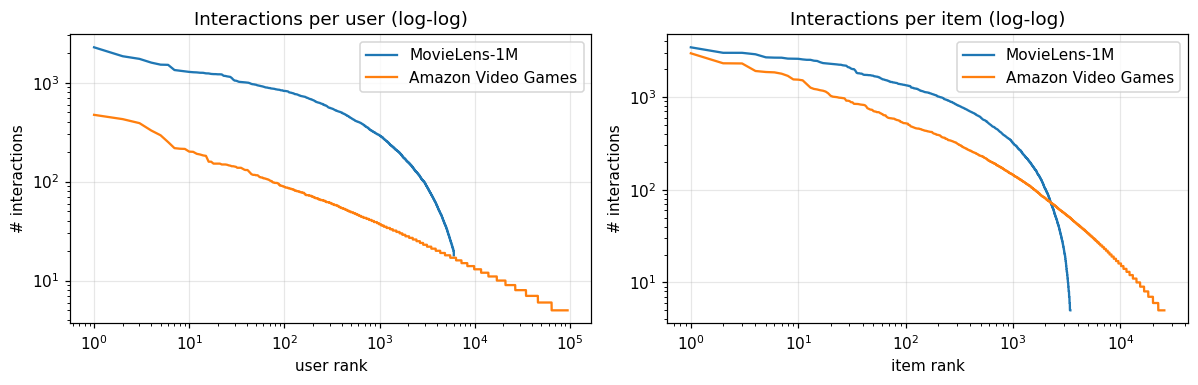
\includegraphics[width=\textwidth]{longtail.png}
\caption{Interactions per user (left) and per item (right), log-log.}
\label{fig:longtail}
\end{figure}

\subsection{Protocol}

We evaluate by \emph{full ranking}: for each user, all items not seen in
training are scored and Recall@$K$ / NDCG@$K$ ($K\in\{10,20\}$) are computed
on the held-out items; no sampled-negative evaluation is used, as it is known
to bias comparisons. Model selection uses validation NDCG@10 with early
stopping (patience 30 epochs). The training budget is 300 epochs for MF
(which always early-stops far below it) and 600 for LightGCN; the reason for
the larger budget is discussed in Section~\ref{sec:ablation}. The full queue
of 18+ runs completes in $\approx$1.5\,h on one NVIDIA L4 GPU.

\section{Results and Analysis}

\subsection{Main comparison}

\begin{table}[h]\centering
\begin{tabular}{llrrrrr}
\toprule
Dataset & Model & R@10 & N@10 & R@20 & N@20 & Best ep. \\
\midrule
MovieLens-1M & MF-BPR & 0.1560 & 0.2456 & 0.2384 & 0.2525 & 45 \\
 & LightGCN ($L{=}3$) & 0.1728 & 0.2605 & 0.2638 & 0.2709 & 450 \\
 & \emph{relative gain} & +10.8\% & +6.1\% & +10.6\% & +7.3\% & \\
\midrule
Video Games & MF-BPR & 0.0634 & 0.0344 & 0.0969 & 0.0431 & 125 \\
 & LightGCN ($L{=}3$) & 0.0907 & 0.0494 & 0.1349 & 0.0608 & 565 \\
 & \emph{relative gain} & +43.2\% & +43.5\% & +39.3\% & +41.2\% & \\
\bottomrule
\end{tabular}

\caption{Test-set results at $d{=}64$ (R = Recall, N = NDCG). LightGCN wins
everywhere, but the relative gain is $\sim$7$\times$ larger on the sparse
dataset.}
\label{tab:main}
\end{table}

Table~\ref{tab:main} shows the central result. On dense MovieLens-1M,
LightGCN improves NDCG@10 by $+6.1\%$; on Video Games the same architecture
change yields $+43.5\%$. The comparison isolates the propagation step as the
only difference, so we conclude that \textbf{the value of higher-order graph
signal grows sharply as direct per-user signal shrinks}. On dense data most
of what the graph could tell the model is already present in each user's own
long history.

\subsection{Convergence behaviour}

\begin{figure}[h]\centering
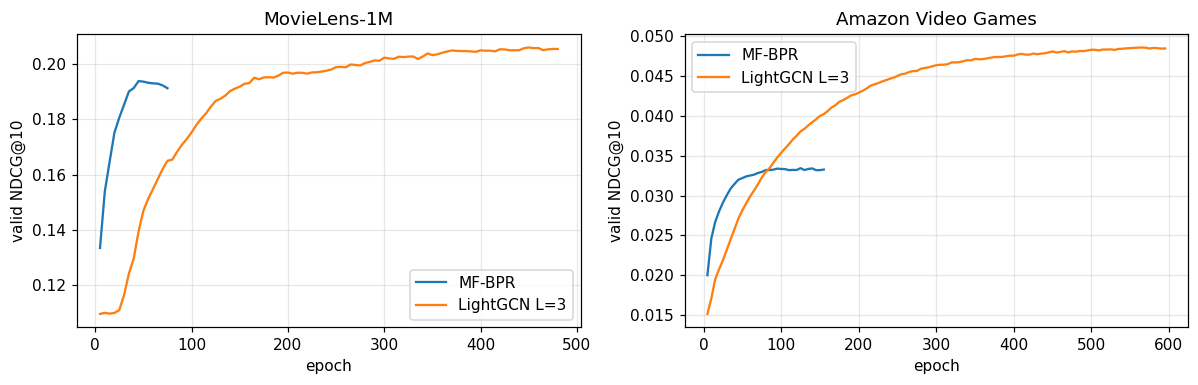
\includegraphics[width=\textwidth]{convergence.png}
\caption{Validation NDCG@10 per epoch. MF converges fast and early-stops
(best epoch 45/125); LightGCN converges $\sim$10$\times$ slower (best epoch
450/565) but reaches a higher plateau.}
\label{fig:convergence}
\end{figure}

Figure~\ref{fig:convergence} shows the cost of the graph: LightGCN needs both
a full-graph propagation per optimization step \emph{and} many more epochs.
On Video Games the two curves cross around epoch 90 --- before that, MF is
the better model. In compute-constrained settings this trade-off matters as
much as the final number.

\subsection{Ablation: propagation depth, and a training-budget pitfall}
\label{sec:ablation}

\begin{figure}[h]\centering
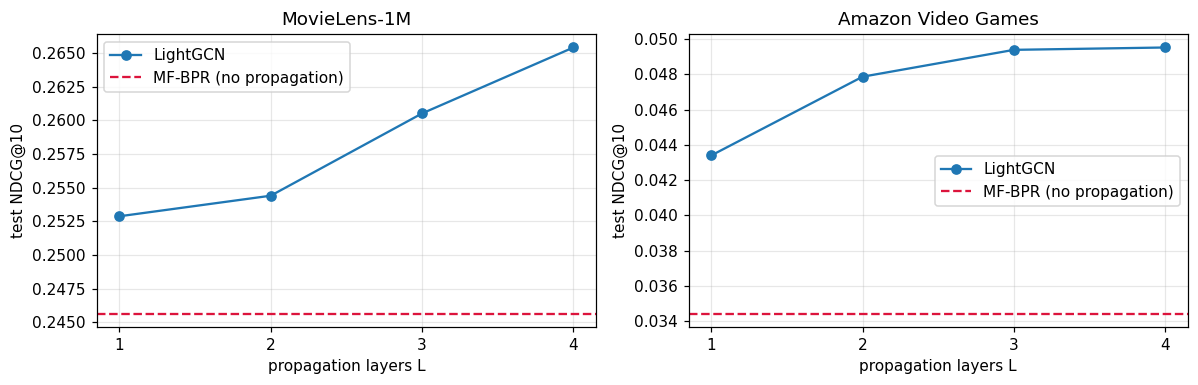
\includegraphics[width=\textwidth]{ablation_layers.png}
\caption{Test NDCG@10 vs.\ propagation layers $L$, all configurations trained
with the same fair 600-epoch budget. Even $L{=}1$ clearly beats MF; no
over-smoothing is visible up to $L{=}4$.}
\label{fig:ablation}
\end{figure}

The layer count $L$ is LightGCN's key component: $L{=}0$ recovers MF, so
Figure~\ref{fig:ablation} directly measures the marginal value of each
propagation hop. Two observations. First, a single hop already captures most
of the gain on the sparse dataset ($+26\%$ NDCG@10 over MF), with diminishing
returns after $L{=}3$. Second --- and this is a finding we consider as
valuable as the curve itself --- our \emph{initial} run of this ablation used
a 300-epoch budget for every $L$ and showed the classic ``peak at shallow
$L$, degradation at $L{=}4$'' pattern commonly attributed to over-smoothing.
Doubling the budget removed the degradation entirely: the best epoch grows
from 110 at $L{=}1$ to $\sim$565 at $L{=}4$, i.e.\ \textbf{deeper propagation
converges more slowly, and an unfair training budget masquerades as
over-smoothing}. Ablation tables in the literature that fix a single epoch
budget across depths should be read with this caveat in mind.

\subsection{Embedding dimension}

\begin{figure}[h]\centering
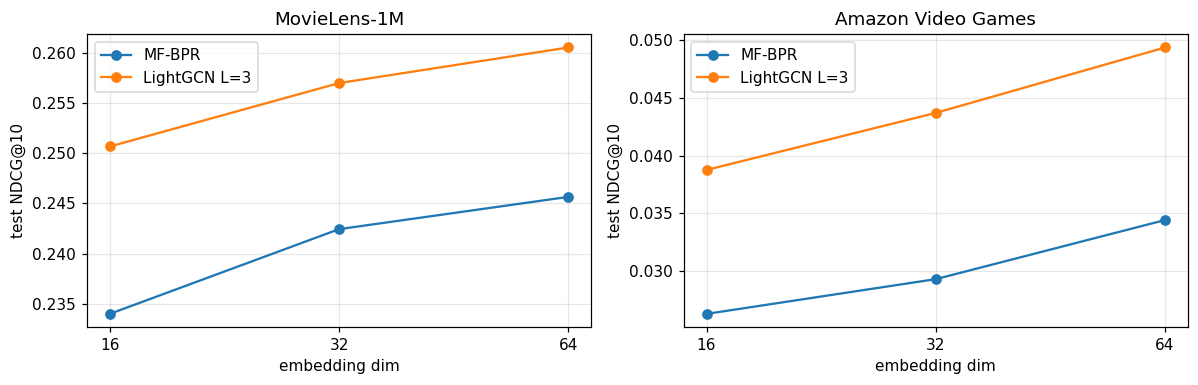
\includegraphics[width=\textwidth]{dim_sweep.png}
\caption{Test NDCG@10 vs.\ embedding dimension $d\in\{16,32,64\}$.}
\label{fig:dims}
\end{figure}

Both methods improve monotonically with $d$ (Figure~\ref{fig:dims}), and the
LightGCN curve is shifted upward roughly in parallel. Notably,
\textbf{LightGCN at $d{=}16$ beats MF at $d{=}64$ on both datasets} despite
having a quarter of the parameters: the graph prior contributes more than raw
capacity does in this regime.

\subsection{Who benefits? Per-user analysis}

\begin{table}[h]\centering
\begin{tabular}{llrrr}
\toprule
Dataset & Train inter. & MF-BPR & LightGCN & Gain \\
\midrule
MovieLens-1M & 14--35 & 0.2877 & 0.3299 & +14.6\% \\
 & 36--75 & 0.2711 & 0.3055 & +12.7\% \\
 & 76--164 & 0.2257 & 0.2442 & +8.2\% \\
 & $\geq$165 & 0.1707 & 0.1775 & +4.0\% \\
\midrule
Video Games & 3--3 & 0.0932 & 0.1335 & +43.3\% \\
 & 4--6 & 0.0962 & 0.1348 & +40.1\% \\
 & $\geq$7 & 0.1020 & 0.1367 & +34.0\% \\
\bottomrule
\end{tabular}

\caption{Recall@20 by user-activity bucket (number of training
interactions). The relative gain shrinks monotonically as activity grows.}
\label{tab:activity}
\end{table}

\begin{figure}[h]\centering
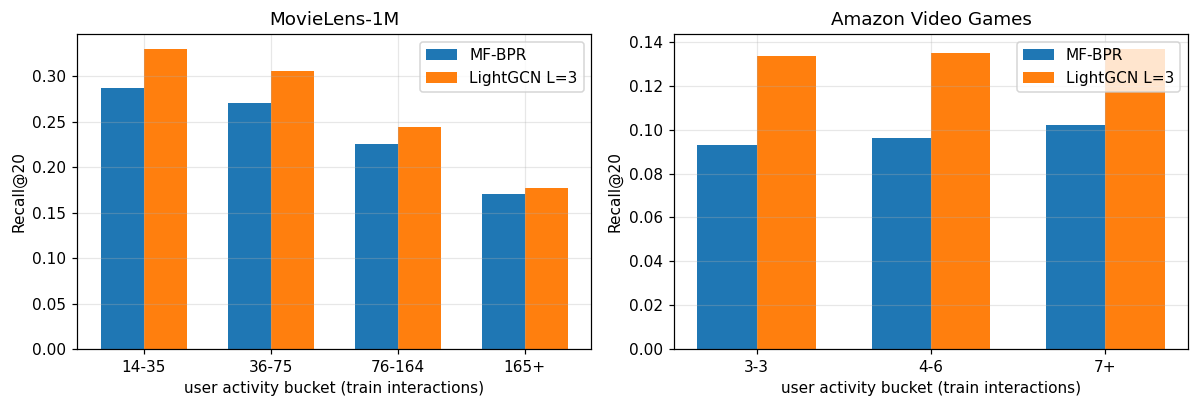
\includegraphics[width=\textwidth]{activity_buckets.png}
\caption{Recall@20 per activity bucket, corresponding to
Table~\ref{tab:activity}.}
\label{fig:activity}
\end{figure}

Bucketing test users by their training degree (Table~\ref{tab:activity},
Figure~\ref{fig:activity}) explains where the improvement lives: on
MovieLens-1M the gain falls monotonically from $+14.6\%$ for the coldest
quartile to $+3.9\%$ for the most active one. Propagation lets a cold user
borrow the histories of neighboring users; a heavy user's own history already
positions them well, and the borrowed signal adds little. A case study makes
this concrete (notebook, Section~6.3): for a sampled 476-interaction user,
MF places \emph{seven} held-out movies in its top-10 versus LightGCN's four
--- averaging in neighborhood signal can actually dilute an already
well-determined profile.

\subsection{Popularity bias and catalog coverage}

\begin{table}[h]\centering
\begin{tabular}{llrr}
\toprule
Dataset & Model & Mean popularity & Coverage@10 \\
\midrule
MovieLens-1M & MF-BPR & 1150 & 50.9\% \\
 & LightGCN & 994 & 61.4\% \\
\midrule
Video Games & MF-BPR & 373 & 62.1\% \\
 & LightGCN & 418 & 41.4\% \\
\bottomrule
\end{tabular}

\caption{Mean training popularity of top-10 recommendations and share of the
catalog that ever appears in a top-10 list.}
\label{tab:popularity}
\end{table}

Table~\ref{tab:popularity} reveals that \emph{how} LightGCN wins differs by
regime. On dense MovieLens-1M it recommends \emph{less} popular items than MF
(mean popularity 1150$\rightarrow$994) and covers \emph{more} of the catalog
(51\%$\rightarrow$61\%): the rich graph individualizes users. On sparse Video
Games the opposite happens: propagation over a thin graph concentrates mass
on bestsellers (373$\rightarrow$418) and coverage drops from 62\% to 41\%.
Part of the $+43.5\%$ headline gain is therefore a \emph{popularity bet}. If
the product goal values discovery and long-tail exposure, this is a genuine
weakness of LightGCN in sparse regimes --- and, we believe, the most
promising direction for improving the method.

\section{Discussion: strengths, weaknesses, key factors}

\textbf{MF-BPR} is fast (best epoch within 45--125), simple, trivially
scalable, and surprisingly strong on dense data and heavy users; its weakness
is cold users, for whom it has almost no signal. \textbf{LightGCN} delivers
consistent accuracy gains that concentrate exactly where MF is weakest, and is
remarkably parameter-efficient; its costs are $\sim$10$\times$ slower
convergence, a full-graph propagation per step, and a popularity/coverage
regression on sparse graphs. The key factors affecting performance in our
experiments were, in order: dataset density, training budget (especially for
deeper propagation), propagation depth $L$, and embedding dimension. Sensible
defaults from our sweeps: $L{=}3$, $d{=}64$, with the caveat that $L$ and the
epoch budget must be increased together.

\section{Conclusion}

We compared MF-BPR and LightGCN under a controlled protocol in which graph
propagation is the only moving part. The higher-order signal helps
everywhere but matters most where direct signal is scarce: sparse datasets
and cold users. The gains are real but not free --- slower convergence, more
compute per step, and on sparse data a shift toward popular items that
sacrifices 21 points of catalog coverage. Finally, our layer ablation shows
that training budget can masquerade as over-smoothing, a reminder that
ablations must equalize convergence, not just epochs. Future work: a
popularity-debiasing extension of LightGCN targeted at the sparse regime,
which our analysis suggests is where the headroom lies.

\begin{thebibliography}{9}
\bibitem{bpr} S.~Rendle, C.~Freudenthaler, Z.~Gantner, L.~Schmidt-Thieme.
BPR: Bayesian Personalized Ranking from Implicit Feedback. \emph{UAI}, 2009.
\bibitem{lightgcn} X.~He, K.~Deng, X.~Wang, Y.~Li, Y.~Zhang, M.~Wang.
LightGCN: Simplifying and Powering Graph Convolution Network for
Recommendation. \emph{SIGIR}, 2020.
\bibitem{ngcf} X.~Wang, X.~He, M.~Wang, F.~Feng, T.-S.~Chua. Neural Graph
Collaborative Filtering. \emph{SIGIR}, 2019.
\bibitem{movielens} F.~M.~Harper, J.~A.~Konstan. The MovieLens Datasets:
History and Context. \emph{ACM TiiS}, 2015.
\bibitem{amazon23} Y.~Hou, J.~Li, Z.~He, A.~Yan, X.~Chen, J.~McAuley.
Bridging Language and Items for Retrieval and Recommendation.
arXiv:2403.03952, 2024.
\end{thebibliography}

\end{document}
